\section{Universal Asynchronous Receiver-Transmitter}

The \emph{Universal Asynchronous Receiver-Transmitter}
protocol, or UART for short, is a
simple, two-wire protocol for
exchanging serial data.

\begin{itemize}
    \item Universal: programmable for different use cases
    \item Asynchronous: sender provides
          no clock signal to receivers
\end{itemize}

UART can be used for communication
between multiple MCUs, and MCU and
its peripherals, or an MCU and PC.
The FTD232 is a converter chip that
converts UART to a standard USB
interface. UART has a start bit and
stop bit for each "frame" of data it
sends, to help with asynchronous
transfer. It also has a parity bit
to help compensate for noise. If using
odd parity, all the \texttt{1}s
(including the parity bit)
must add up to an odd number. Vice
versa for even parity. More advanced
error correction codes like Hamming
or Reed-Solomon can detect or fix
multiple bit flips, but these are
outside the scope of this course.

The \emph{baud} rate is the maximum
rate of signal transitions per second
for a serial communication system.
The Baud rate is not the rate at which
data is transmitted. It conveys how
fast the signal changes, but not all
signal changes convey meaningful data.
For instance, if we have a start
and stop bit, along with a parity bit,
and five bits of data, then the data
rate is only $\frac{5}{8}$ of the Baud
rate.

RS-232 sets the recommended
standard for UART.
In the standard UART protocol,
we make sure that the data line is
kept high when idle, and use 0 as
the start bit. Data bits are sent
LSB first. Parity can be odd, even,
or neither. The stop bit goes high.
In UART, there is always a start
bit. Word size ranges from 7 to 9
bits. Parity bit is option and can
be even or odd. There is always a
stop signal, but it can be 0.5, 1,
1.5, or 2 bit widths long. Almost
everyone in the world uses 8N1, which
is eight bits, no parity, one stop
bit. UART has a sending pin (Tx) and a
receiving pin (Rx). Both Tx and Rx can be
active at the same time and independently,
as seen in Figure \ref{fig:uart}.

\begin{figure}
    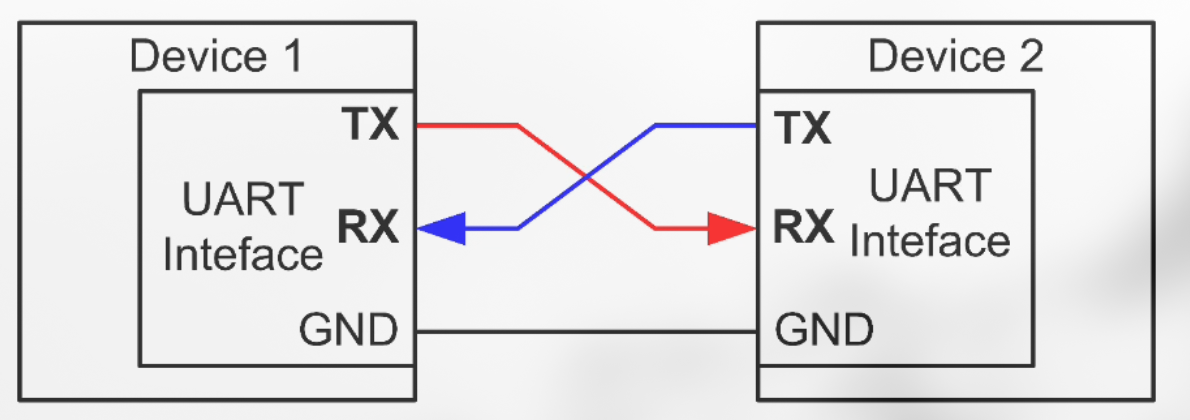
\includegraphics{images/uart.png}
    \caption{UART}
    \label{fig:uart}
\end{figure}

No two clocks are the same.
In UART, clocks sync on the
falling edge of the start bit.
There's a 1.5-bit duration wait
to read the data and each new
bit is read one bit-duration
later. The clocks are resynced
on the next start bit. The
Baud rate of the receiver is
allowed to differ from that of
the transmitter by up to
5\%. If each bit is shifted by 5\%,
then each successive bit will be
a little later or a little
earlier. This has a cumulative
effect. $10.5^8 = 1.477$,
still not beyond halfway at
the 8th bit, but $1.05^9 = 1.551$,
just over halfway at the 9th bit.
